The followed informations introduce the results of two different tests. 
To make both tests, they were used the images available by KITTI\cite{Geiger}.


In the first test, see Fig. \ref{fig:imgpapercerta}, 
the algorithm makes the tracking of an object through of 9 images with 
a displacement approximately perpendicular to the observer (approximately 2D displacement).
\begin{figure}[!hbt]
\centering
  \subfloat[]{\label{fig:imgpapercertaa} \includegraphics[width=.48\columnwidth]{images/images/0000000000.png}}
  \subfloat[]{\label{fig:imgpapercertab} \includegraphics[width=.48\columnwidth]{images/images/img_paper_certa.eps}}
  \caption{The image in (a) represents the target in your initial position 
   and the image (b) shows the vehicle in your final position.}
  \label{fig:imgpapercerta}
\end{figure}
The initial position of object is in the image (a) and the final position in (b); 
also, it is generated a vector that  illustrates the tracking made by the algorithm.
We can observe that there is a small bend in the image 
and it generates a slight change of object perspective. 
This cause the update of $ROI$, which involves seeing a slight change in area.
The difference among initial and final value of the departure factor may 
be considered small, as can be seen in the Fig \ref{fig:res_graph1};
but, should put us on attention to improve the method of calculating the area,
to discount areas that do not belong to the object.
\begin{figure}[!hbt]
\centering
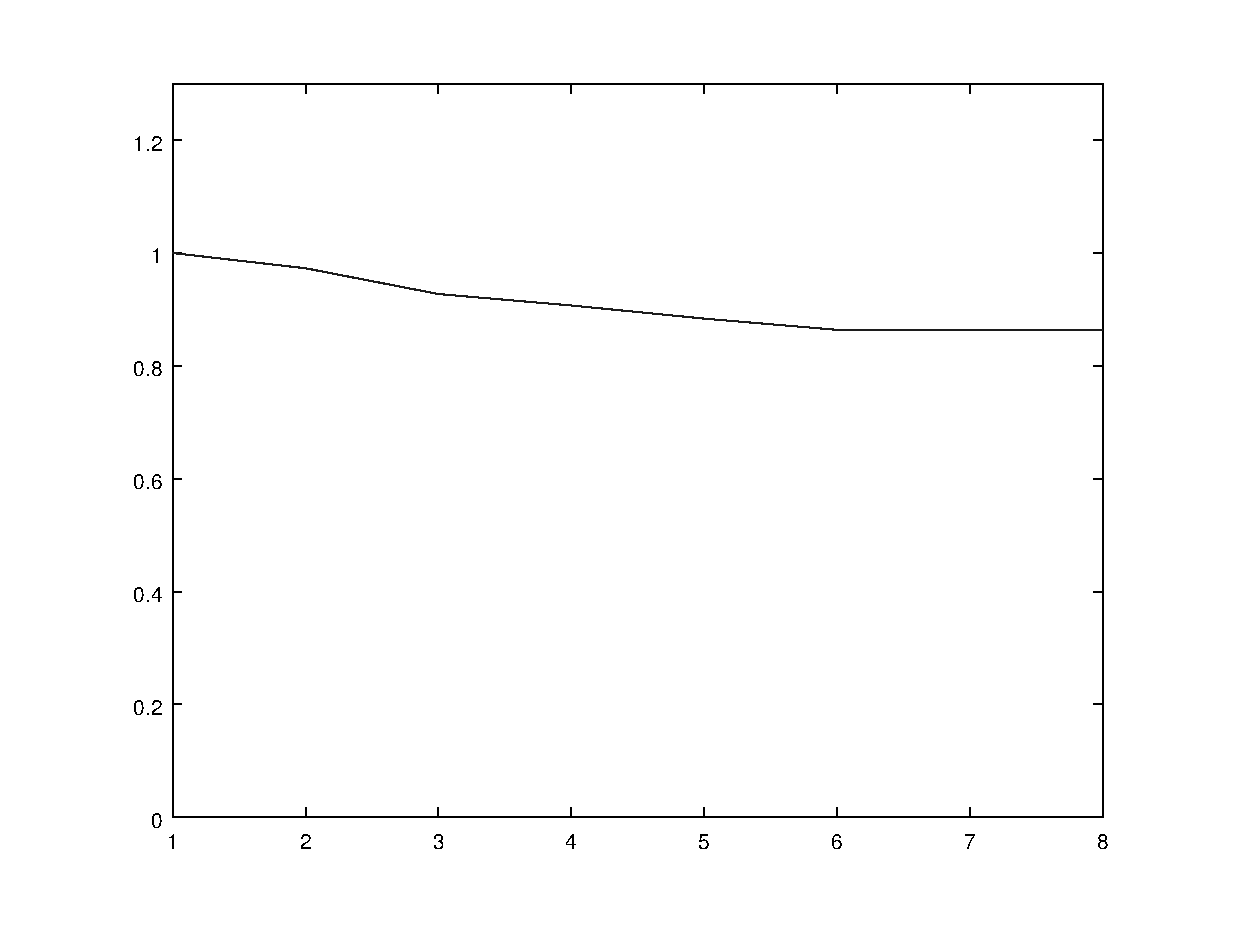
\includegraphics[width=0.8\columnwidth]{images/graph1.eps}
\caption{Departure factor for each frame in the test 1.}
\label{fig:res_graph1}
\end{figure}
The Fig. \ref{fig:res_graph1v} shows the velocity of departure factor
to a value $d_0=1$ and a $\Delta t=1$. It is easy to see that the variation,
between frames, of departure factor is very small when compared with 1, 
having a mean departure factor velocity of $-0.017020$. This imply a mean approach of $1.7\%$ of $d_0$
in each one of 9 frames.
\begin{figure}[!hbt]
\centering
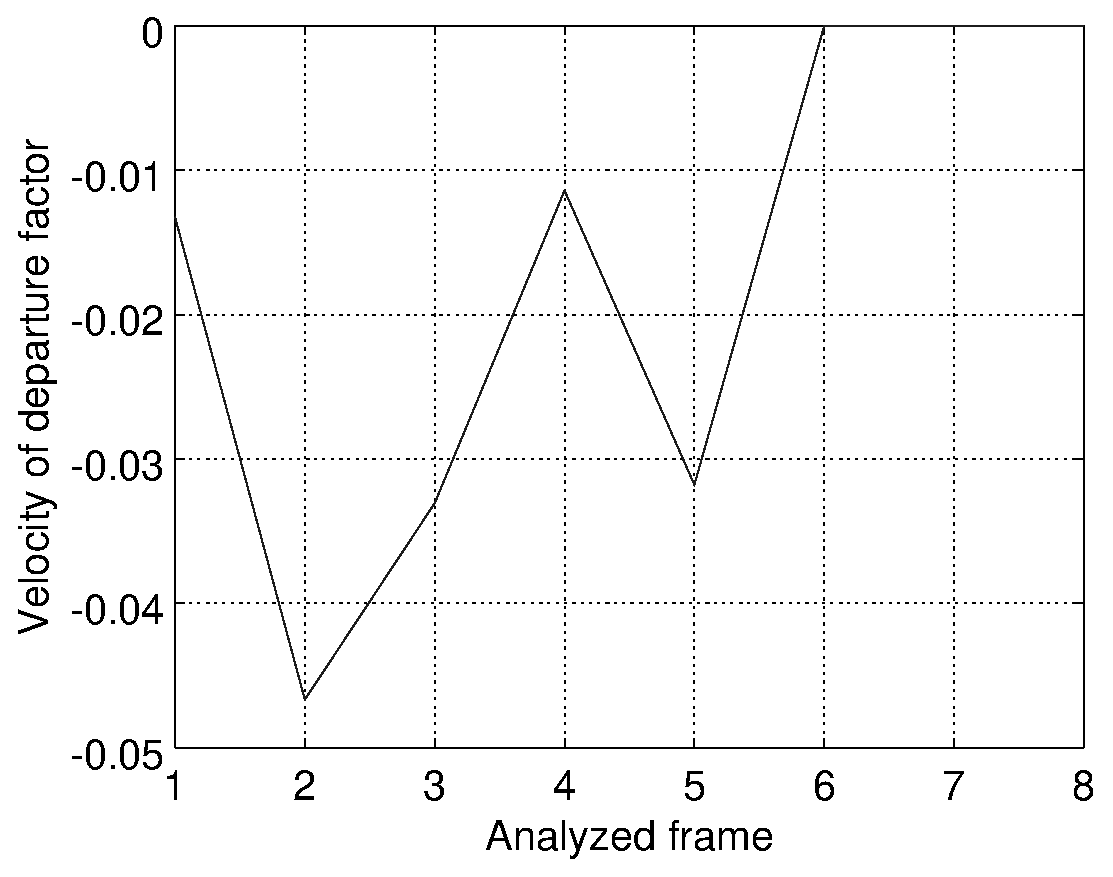
\includegraphics[width=0.8\columnwidth]{images/graph1v.eps}
\caption{Velocity of departure factor for each frame in the test 1.}
\label{fig:res_graph1v}
\end{figure}


In the second test, we prove the functionality of algorithm in 3D. 
The program compares the images and calculates the departure factor 
based on the object area. The Fig. \ref{fig:target} demonstrates the 
tracking of $100$ images from initial at the final position of target, 
highlighted with red boxes;
where, the vector in blue color describes the movement of object. 
\begin{figure}[!hbt]
\centering
  \subfloat[]{\label{fig:targeinit} \includegraphics[width=.48\columnwidth]{images/images/351.jpg}}
  \subfloat[]{\label{fig:targeend} \includegraphics[width=.48\columnwidth]{images/graph2p.eps}}
  \caption{The object in (a) is the initial position and its area is 
  fewer than the figure in (b), which is in final position. 
  The factor is calculate dividing both areas.}
  \label{fig:target}
\end{figure}
In the figure, we can observe a significant increase in the area of vehicle. 
So, your influence in the departure factor can be seen in the Fig. \ref{fig:res_graph2}.

\begin{figure}[!hbt]
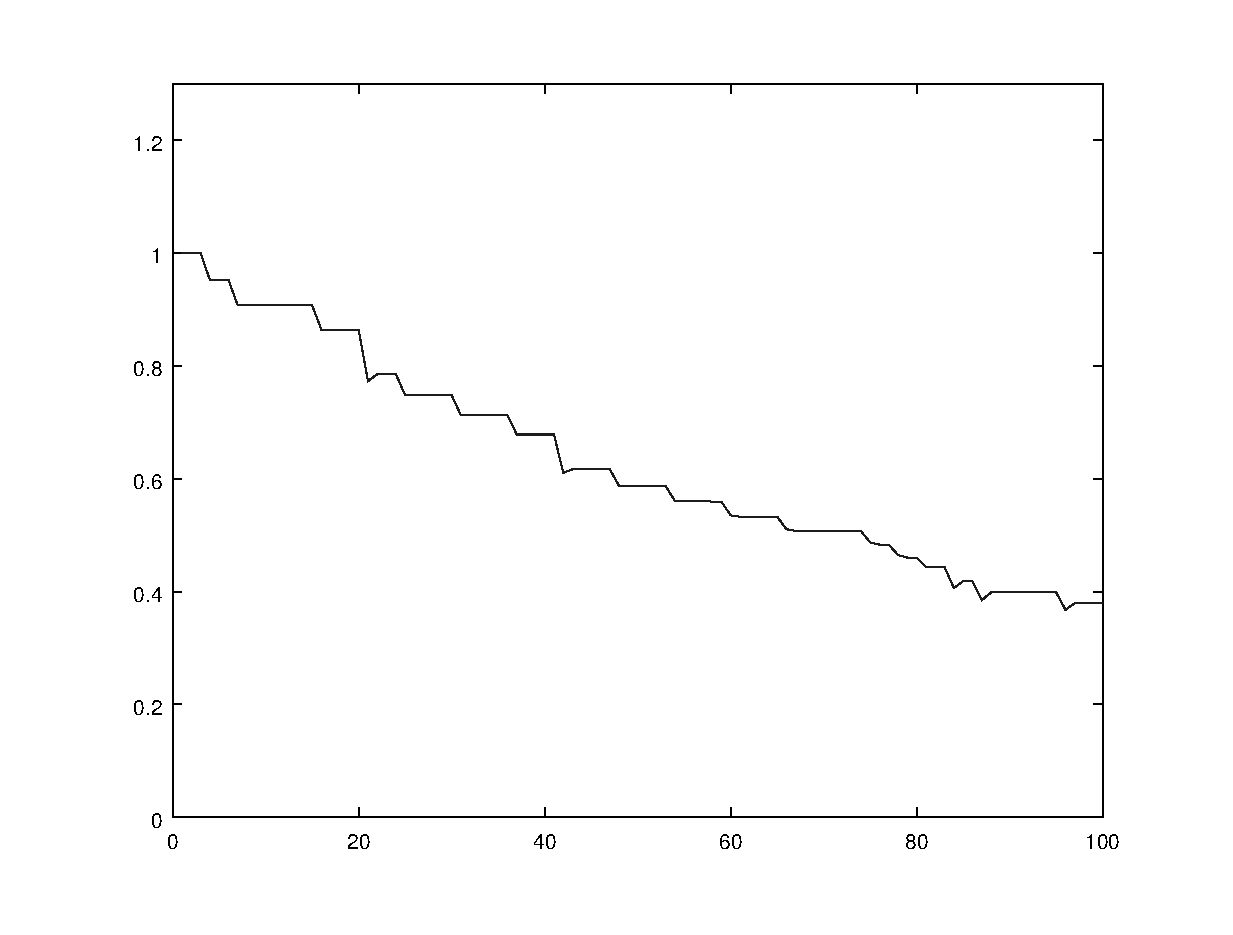
\includegraphics[width=\columnwidth]{images/graph2.eps}
\caption{Departure factor for each frame in the test 2.}
\label{fig:res_graph2}
\end{figure}
The graphic shows the departure factor in each frame
of test 2, if we interpret this value as the position in each sample time, 
then the departure factor describes the relative target position.
So that, in the first image the analyzed object is at a distance $d_0$ 
and in the last image the object is at a distance of $52.42\%$ of $d_0$.
The departure distance decreases in discrete steps because the departure
factor is selected also in discrete steps, so that if the target is
between two consecutive analysis layers (scales), then the algorithm
approximates the target to the nearest layer. 
\begin{figure}[!hbt]
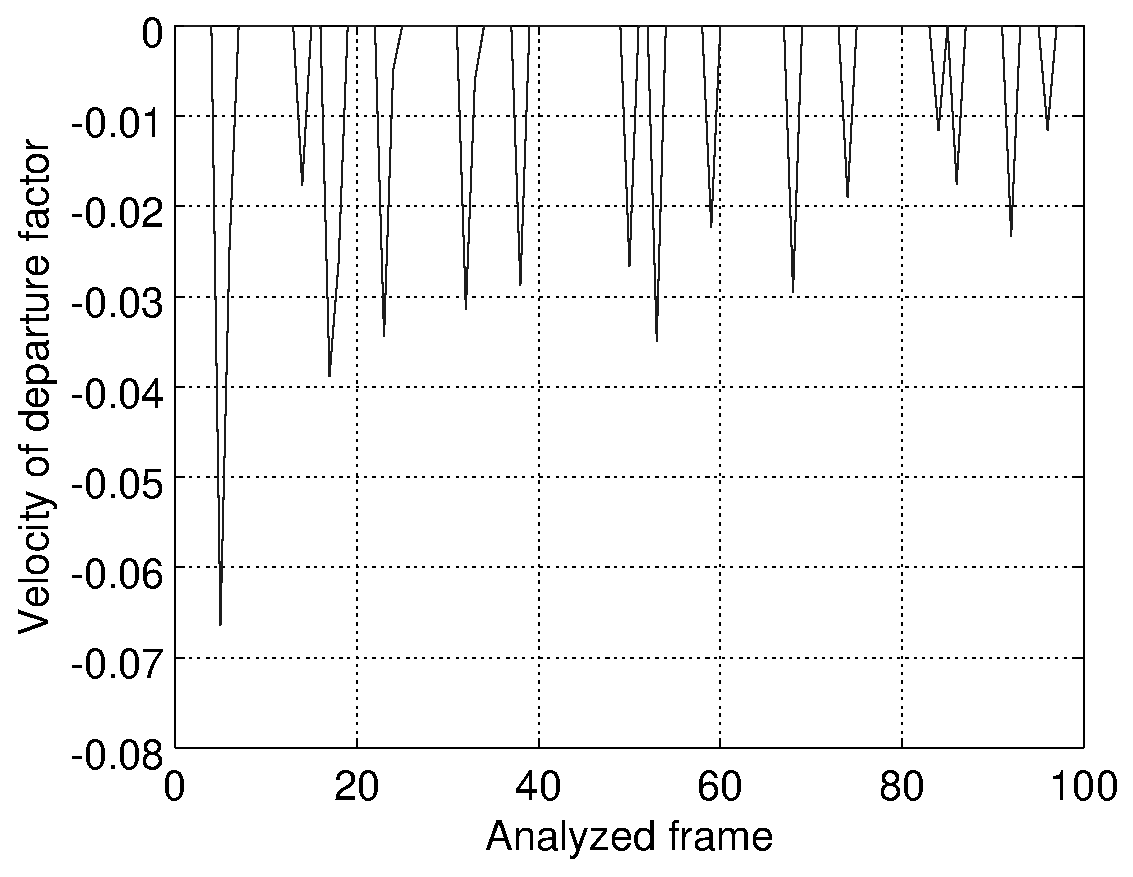
\includegraphics[width=\columnwidth]{images/graph2v.eps}
\caption{Velocity of departure factor for each frame in the test 2.}
\label{fig:res_graph2v}
\end{figure}
By other side, the velocity of departure factor can be seen in the 
Fig. \ref{fig:res_graph2v}, where the velocity is calculated
to $d_0=1$ and $\Delta t=1$. The mean value of the departure
velocities is equal to $-0.0048$, it indicates that the
analyzed object is in approaching to the observer. Similarly
to the case of test 1, this mean velocity can be interpret
as a mean approach of $0.48\%$ of $d_0$, in each one of 100 frames.
If we compare the test 1 and 2 to the same $\Delta t=1$, is easy to see
that the departure velocity of test 2  is lower than the test 1, 
but as the test 2 has more analyzed frames (100 images)
and because this the approaching to the observer is greater; 
not to mention that in the test 1, the small number of images 
make  unrepresentative the mean value.




